% Chapitres 1-9 - Tous les faits verifies contre le codebase

% ======================== CHAPITRE 1 ========================
\section{Chapitre 1 : Rappels}

\subsection{D\'efinitions Fondamentales}

Avant d'aborder les concepts avanc\'es du G\'enie Logiciel, il est essentiel de poser les bases terminologiques et conceptuelles.

\subsubsection{Logiciel et Application}

Un \textbf{logiciel} est d\'efini comme un ensemble de programmes, proc\'edures, r\`egles et documentations relatifs au fonctionnement d'un ensemble de traitements d'informations. Une \textbf{application} est un logiciel qui sert \`a implanter un syst\`eme d'informations. On distingue trois grandes cat\'egories : applications de gestion (peu de traitement, beaucoup de donn\'ees), applications scientifiques (beaucoup de traitement, peu de donn\'ees), et applications industrielles (peu de traitement et de donn\'ees).

SaaS Directory s'inscrit dans la cat\'egorie des applications de gestion/web, avec une composante significative de donn\'ees structur\'ees (20 tables relationnelles).

\subsubsection{Syst\`eme d'Information (SI)}

Le \textbf{Syst\`eme d'Information (SI)} constitue l'ensemble des flux d'op\'erations, d'informations et de moyens mis en oeuvre par une organisation. Le \textbf{Syst\`eme d'Information Automatis\'e (SIA)} repose sur la technologie informatique. SaaS Directory est un SIA complet : il traite des profils utilisateurs, des produits, des votes, des messages et des abonnements via une infrastructure web moderne.

\subsubsection{M\'ethode, Outil et M\'ethodologie}

\begin{definitionbox}[title={D\'efinition : M\'ethode (Grady Booch, 1994)}]
Une m\'ethode est un processus disciplin\'e qui g\'en\`ere un ensemble de mod\`eles d\'ecrivant les diff\'erents aspects d'un syst\`eme logiciel, en utilisant une notation bien d\'efinie.
\end{definitionbox}

Un \textbf{outil} d\'esigne un programme ou un ensemble de programmes aidant \`a la mise en oeuvre des techniques. L'\textbf{Atelier de G\'enie Logiciel (AGL)} regroupe l'ensemble des outils utilis\'es pour le d\'eveloppement, la maintenance et la documentation.

La \textbf{m\'ethodologie} est la d\'emarche g\'en\'erale qui fait appel \`a des m\'ethodes et des outils pour aboutir au logiciel final. Pour SaaS Directory, la m\'ethodologie adopt\'ee combine l'approche incrémentale it\'erative avec les principes du cycle de vie en V.

\subsection{Application \`a SaaS Directory}

SaaS Directory s'inscrit dans le cadre th\'eorique des Syst\`emes d'Information Automatis\'es. En tant que marketplace web, il traite de grands volumes de donn\'ees structur\'ees et exige une architecture logicielle rigoureuse pour garantir performance, s\'ecurit\'e et \'evolutivit\'e.


% ======================== CHAPITRE 2 ========================
\section{Chapitre 2 : G\'enie Logiciel --- G\'en\'eralit\'es}

\subsection{Objectifs du G\'enie Logiciel}

Le \textbf{G\'enie Logiciel (GL)} vise \`a utiliser l'informatique dans les entreprises comme outil quotidien, \`a r\'eduire les co\^uts de d\'eveloppement et de maintenance, \`a am\'eliorer la qualit\'e des logiciels, et \`a augmenter la productivit\'e des \'equipes. Ces objectifs s'inscrivent dans une d\'emarche globale de ma\^itrise du cycle de vie du logiciel.

\subsection{Les Principes du GL Appliqu\'es}

\subsubsection{Rigueur}

La rigueur se traduit par l'utilisation de TypeScript (typage statique strict), les conventions de nommage syst\'ematiques (PascalCase pour les composants, camelCase pour les fonctions), et la revue de code via les pull requests Git. La documentation interne du projet documente les conventions sp\'ecifiques de d\'eveloppement.

\subsubsection{S\'eparation des Probl\`emes}

Trois niveaux de s\'eparation sont appliqu\'es : s\'eparation dans le temps (d\'eveloppement par phases avec tests \`a chaque niveau), s\'eparation dans l'espace (architecture en couches, voir figure~\ref{fig:layers}), et s\'eparation en sous-syst\`emes (modules application, composants et utilitaires serveur).

\begin{figure}[htbp]
\centering
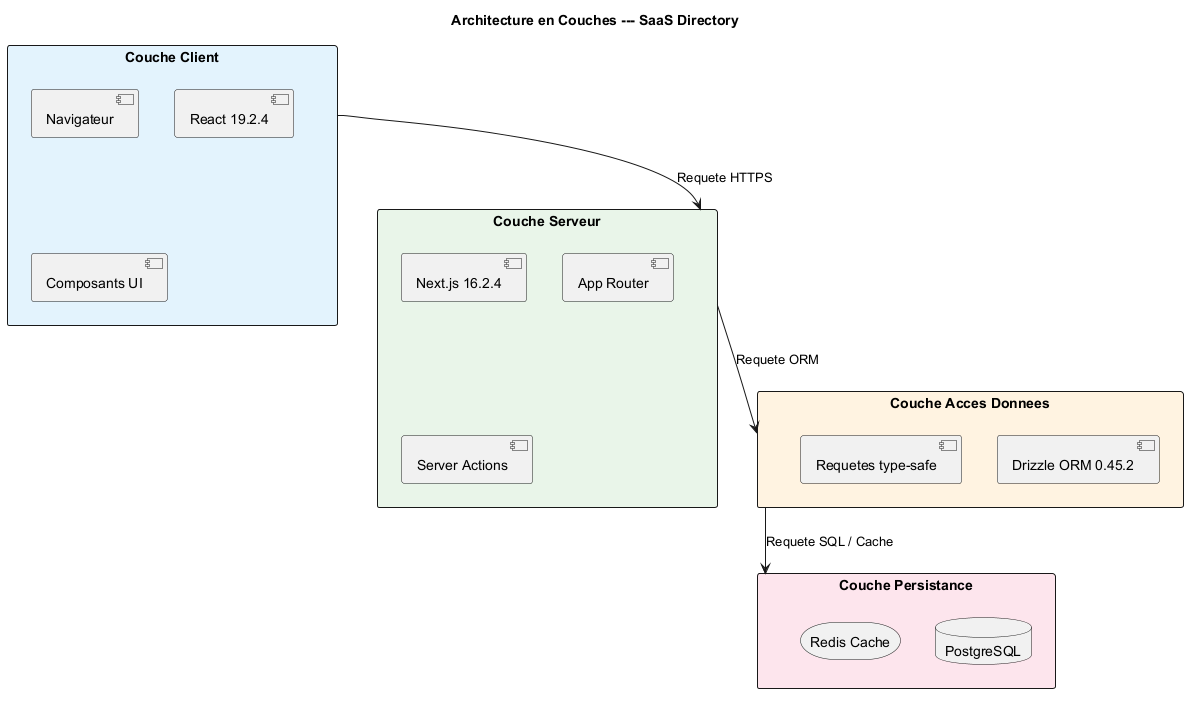
\includegraphics[width=0.85\textwidth,height=0.70\textheight,keepaspectratio]{assets/architecture_layers.png}
\caption{Architecture en Couches --- SaaS Directory}
\label{fig:layers}
\end{figure}

\subsubsection{Modularit\'e}

L'architecture repose sur des composants React ind\'ependants, chacun responsable d'une fonctionnalit\'e sp\'ecifique. Le sch\'ema Drizzle ORM d\'ecompose le syst\`eme en 20 tables distinctes, chacune encapsulant une entit\'e m\'etier. Cette modularit\'e facilite la maintenance et les tests unitaires.

\subsubsection{Abstraction}

Plusieurs niveaux d'abstraction sont utilis\'es : les Server Actions abstraient la logique m\'etier du rendu UI ; Drizzle ORM abstrait les requ\^etes SQL complexes ; le syst\`eme de cache Redis abstrait la gestion des donn\'ees temporaires.

\subsubsection{G\'en\'ericity}

Les composants UI sont con\,cus comme des composants r\'eutilisables param\'etrables via les propri\'et\'es React. Le syst\`eme d'authentification Better Auth est g\'en\'erique et supporte OAuth (Google, GitHub) et l'authentification par email/mot de passe. Le diagramme d'activit\'e de la figure~\ref{fig:auth-activity} illustre le flux complet d'authentification.

\begin{figure}[htbp]
\centering
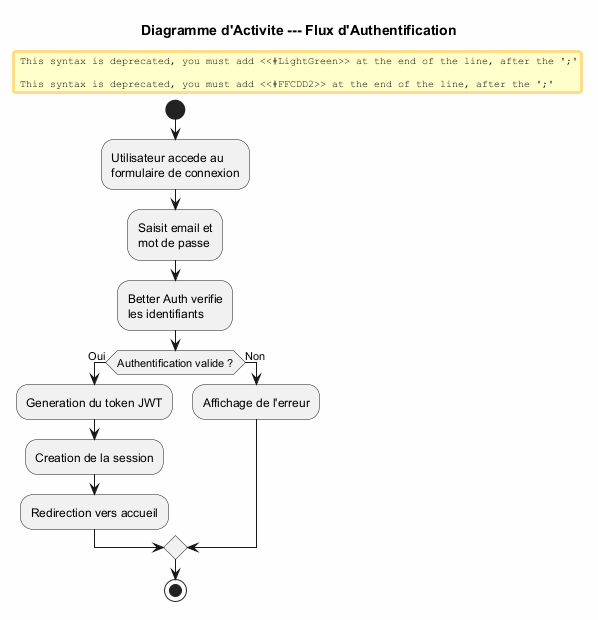
\includegraphics[width=0.90\textwidth,height=0.70\textheight,keepaspectratio]{assets/auth_activity.png}
\caption{Diagramme d'Activit\'e --- Flux d'Authentification}
\label{fig:auth-activity}
\end{figure}

\subsubsection{Construction Incr\'ementale}

Le d\'eveloppement a suivi une approche incrémentale document\'ee dans l'historique Git. Les phases principales sont : fondations (Next.js 16.2.4, shadcn, Drizzle), infrastructure de tests (Vitest, Playwright), base de donn\'ees (sch\'ema Drizzle, migrations, seed), authentification TDD (login/signup, tests), fonctionnalit\'es core (marketplace, profils, messages, notifications), et polissage final (recherche, responsive, build fixes).

\subsubsection{Anticipation du Changement}

L'architecture anticipe plusieurs \'evolutions : le sch\'ema Drizzle inclut d\'ej\`a les champs client et abonnement Stripe pour une future int\'egration du paiement ; le syst\`eme de plans (Free/Pro) permet d'ajouter de nouveaux niveaux d'abonnement. Le diagramme de la figure~\ref{fig:subscription-state} pr\'esente le cycle de vie des abonnements.

\begin{figure}[htbp]
\centering
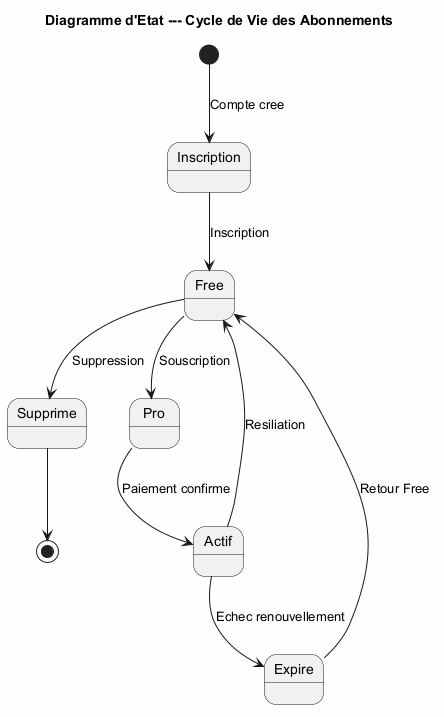
\includegraphics[width=0.90\textwidth,height=0.70\textheight,keepaspectratio]{assets/subscription_state.png}
\caption{Diagramme d'\'Etat --- Cycle de Vie des Abonnements}
\label{fig:subscription-state}
\end{figure}

\subsection{Les Attributs du Logiciel}

L'analyse du codebase de 12 166 lignes r\'eparties sur 108 fichiers permet d'\'evaluer ces attributs.

\subsubsection{Couplage}

Le couplage est faible gr\^ace \`a l'architecture par composants React et l'encapsulation des Server Actions. Chaque table Drizzle ORM est ind\'ependante, avec des relations explicites via les cl\'es \'etrang\`eres. Le couplage entre frontend (React) et backend (Server Actions) est r\'eduit au minimum par l'API interne de Next.js 16.2.4.

\subsubsection{Complexit\'e}

Avec 20 tables relationnelles et 12 166 lignes de code, le syst\`eme pr\'esente une complexit\'e mod\'er\'ee. Cette complexit\'e est ma\^itrisee par la modularit\'e, le typage statique TypeScript, et la documentation inline (JSDoc).

\subsubsection{Extensibilit\'e}

L'extensibilit\'e est d\'emontr\'ee par la facilit\'e d'ajouter de nouvelles tables au sch\'ema Drizzle (4 migrations versionn\'ees), l'ajout de nouveaux composants UI sans impacter les existants, et la configuration modulaire du framework.

\subsubsection{Lisibilit\'e et Visibilit\'e du Comportement}

La lisibilit\'e est assur\'ee par TypeScript (typage explicite), les conventions de nommage strictes, et la documentation JSDoc. La visibilit\'e du comportement est garantie par les tests unitaires (10 fichiers de test couvrant l'authentification, la souscription, le sch\'ema, les actions serveur) et les tests end-to-end (Playwright 1.59.1).


% ======================== CHAPITRE 3 ========================
\section{Chapitre 3 : Repr\'esentations du Cycle de Vie du Logiciel}

Le d\'eveloppement d'un logiciel n'est pas simplement l'\'ecriture d'un programme. La taille et la complexit\'e des logiciels actuels exigent l'utilisation de processus de d\'eveloppement structur\'es, appel\'es \textbf{cycles de vie du logiciel}.

\subsection{Les Mod\`eles de Cycle de Vie}

Le mod\`ele en cascade (waterfall) suit une s\'equence lin\'eaire de phases : sp\'ecification, conception, codage, tests, et maintenance. Le mod\`ele en V associe \`a chaque phase de d\'eveloppement une phase de test correspondante. Le mod\`ele it\'eratif et incr\'emental divise le projet en it\'erations courtes, chacune livrant une version fonctionnelle du logiciel.

\subsection{Choix et Justification du Mod\`ele}

Pour SaaS Directory, nous avons adopt\'e un \textbf{mod\`ele hybride} combinant l'approche incr\'ementale it\'erative avec des \'el\'ements du mod\`ele en V. Cette d\'ecision repose sur trois arguments : la nature \'evolutive du projet (marketplace web), les contraintes temporelles acad\'emiques, et l'importance de la validation syst\'ematique (tests \`a chaque niveau).

\subsection{Application au Projet SaaS Directory}

Le d\'eveloppement de SaaS Directory s'est d\'eroul\'e sur environ trois semaines, du 5 au 21 mai 2026, comme l'atteste l'historique Git du projet. Le travail a \'et\'e r\'eparti entre trois d\'eveloppeurs selon une approche incr\'ementale it\'erative.

\textbf{Phase 1 : Fondations (5 mai).} Initialisation du projet Next.js 16.2.4 avec TypeScript et Tailwind CSS v4, configuration de Drizzle ORM 0.45.2 avec PostgreSQL, mise en place de Better Auth 1.6.9, et cr\'eation des tables de base (user, session, account, verification).

\textbf{Phase 2 : Infrastructure de tests (5--6 mai).} Mise en place de Vitest 4.1.5, React Testing Library, Playwright 1.59.1, et configuration des seuils de couverture.

\textbf{Phase 3 : Base de donn\'ees et sch\'ema (6 mai).} D\'efinition du sch\'ema Drizzle ORM complet (20 tables), cr\'eation des 4 migrations versionn\'ees, et script de seed.

\textbf{Phase 4 : Authentification et profils (6 mai).} D\'eveloppement des pages login/signup avec TDD, gestion des profils utilisateurs, et syst\`eme de lancement de produits.

\textbf{Phase 5 : Fonctionnalit\'es core (6--7 mai).} D\'eveloppement du marketplace (votes, commentaires), messagerie en temps r\'eel, et syst\`eme d'abonnements Free/Pro.

\textbf{Phase 6 : Polissage et optimisation (7--8 mai, 21 mai).} Ajout de la recherche, reset de mot de passe, pagination infinie, corrections responsive, et build fixes.


% ======================== CHAPITRE 4 ========================
\section{Chapitre 4 : La D\'emarche}

La d\'emarche de conception d'un logiciel d\'efinit la m\'ethodologie suivie pour passer du besoin exprim\'e au logiciel op\'erationnel.

\subsection{M\'ethodes de D\'eveloppement Semi-Formelles}

Le cours pr\'esente plusieurs m\'ethodes semi-formelles. SADT (Structure Analysis and Design Technique) est une m\'ethode structur\'ee. MERISE est une m\'ethode fran\,caise syst\'emique avec s\'eparation donn\'ees et traitements. UML/Processus Unifi\'e est it\'eratif, incr\'emental et orient\'e objet. OMT (Object Modelling Technique) a \'et\'e propos\'e par James Rumbaugh. OOSE (Object-Oriented Software Engineering) a \'et\'e d\'evelopp\'e par Ivar Jacobson.

Pour SaaS Directory, nous avons retenu l'approche UML/Processus Unifi\'e pour plusieurs raisons : son caract\`ere it\'erati f et incr\'emental correspond \`a notre mod\`ele de cycle de vie ; son orientation objet s'aligne avec notre stack technologique (React composants, Drizzle ORM entit\'es) ; et UML est le standard industriel de facto pour la mod\'elisation orient\'ee objet.

\subsection{Diagrammes UML Appliqu\'es au Projet}

\subsubsection{Diagramme de Cas d'Utilisation}

Le diagramme de cas d'utilisation mod\'elise les interactions entre les acteurs et le syst\`eme. Les acteurs principaux sont : Visiteur, Utilisateur Authentifi\'e, Cr\'eateur de Produit, et Administrateur.

\begin{figure}[htbp]
\centering
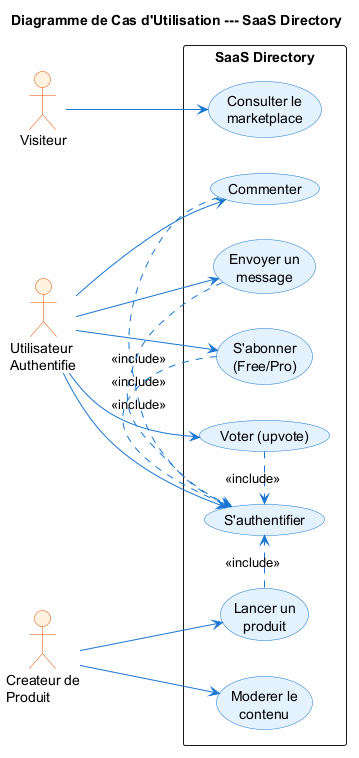
\includegraphics[width=0.95\textwidth,height=0.70\textheight,keepaspectratio]{assets/use_case.png}
\caption{Diagramme de Cas d'Utilisation --- SaaS Directory}
\label{fig:use-case}
\end{figure}

\subsubsection{Diagramme de Classes}

Le sch\'ema Drizzle ORM constitue l'impl\'ementation directe du diagramme de classes. Le syst\`eme compte 20 tables.

\begin{figure}[p]
\centering
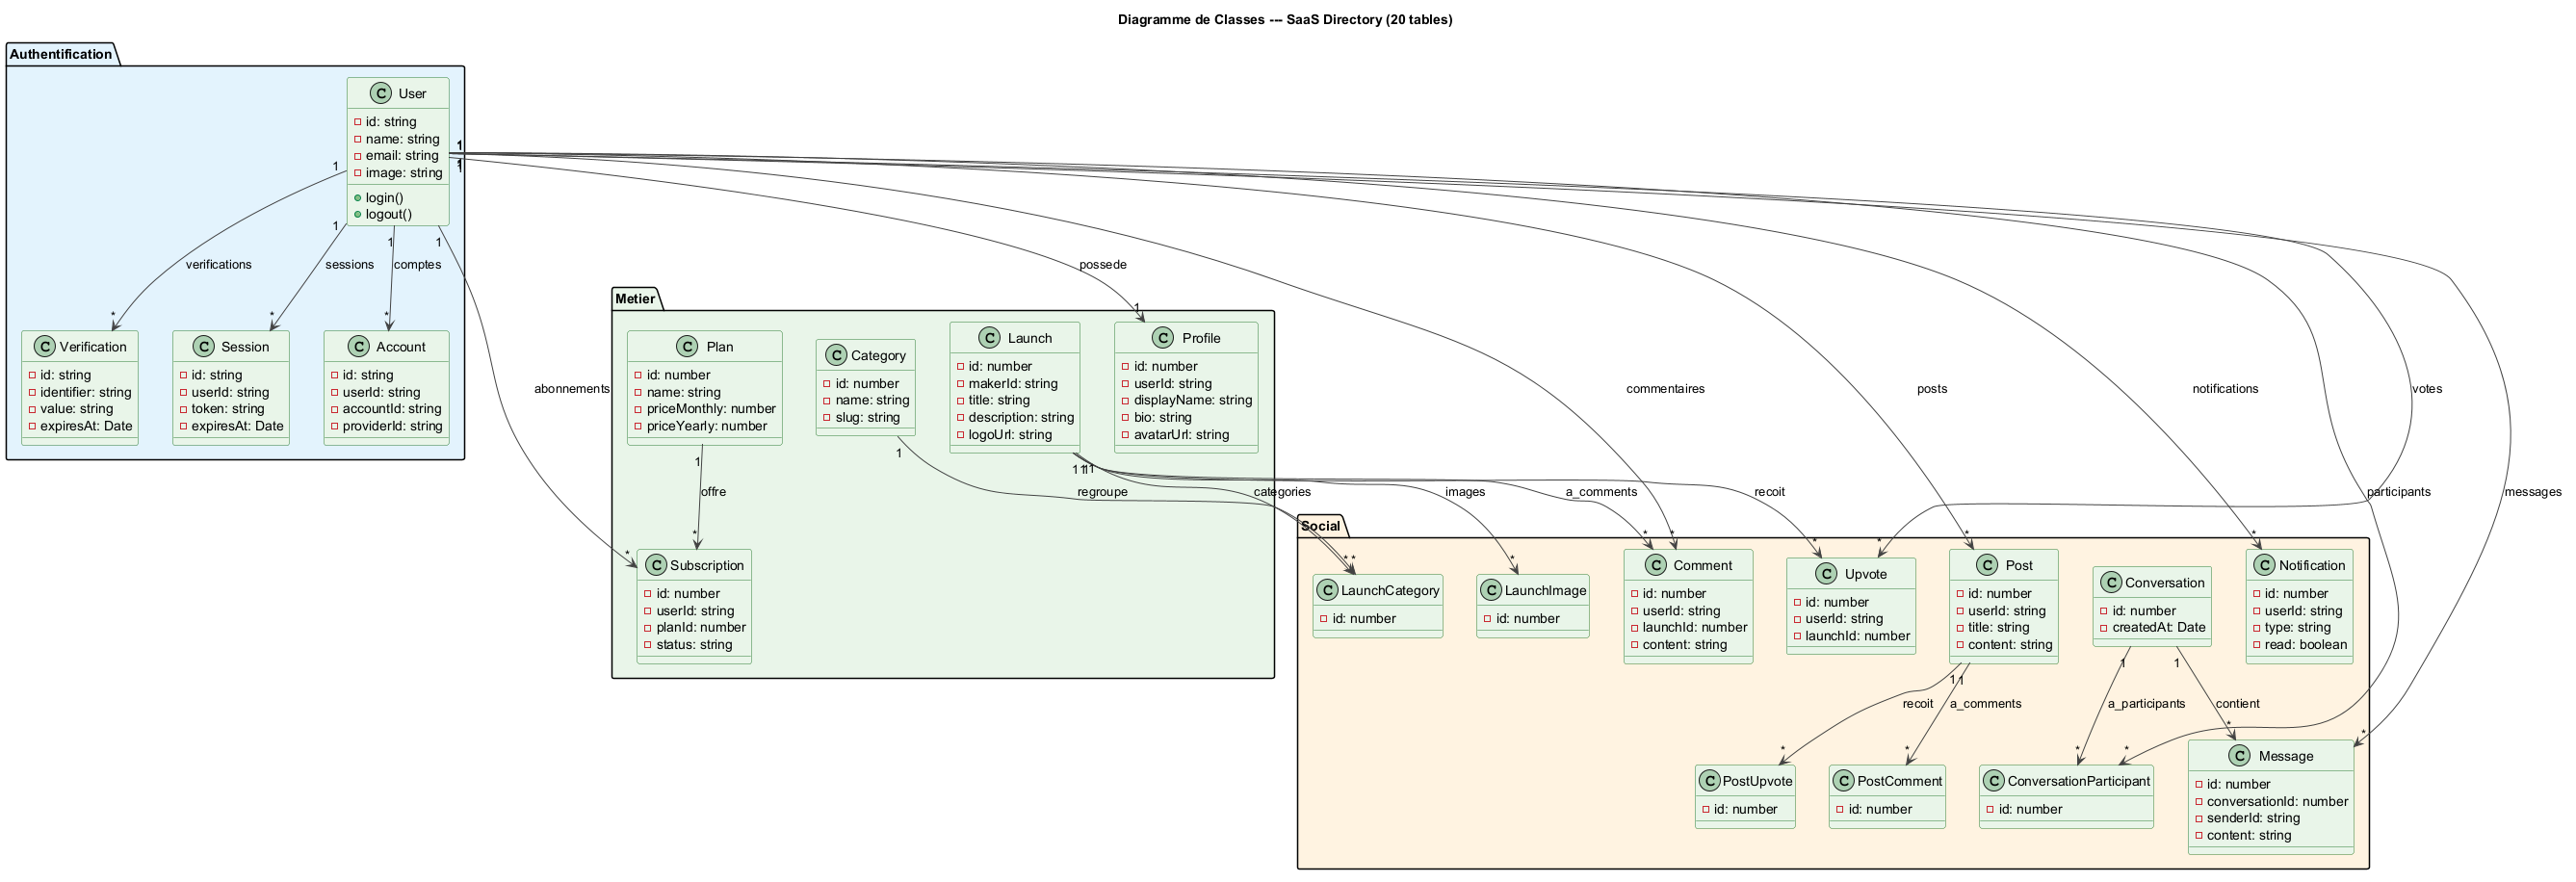
\includegraphics[width=0.90\textwidth,height=0.70\textheight,keepaspectratio]{assets/class.png}
\caption{Diagramme de Classes (20 tables)}
\label{fig:class}
\end{figure}

Les tables sont regroup\'ees en trois cat\'egories : \textbf{Better Auth} (user, session, account, verification) ; \textbf{m\'etier principal} (profile, launch, category, plan, subscription) ; et \textbf{interaction sociale} (upvote, comment, post, postUpvote, postComment, conversation, conversationParticipant, message, notification).

\subsubsection{Diagramme de S\'equence}

Le diagramme de s\'equence illustre l'interaction entre les acteurs et le syst\`eme lors de l'envoi d'un message.

\begin{figure}[htbp]
\centering
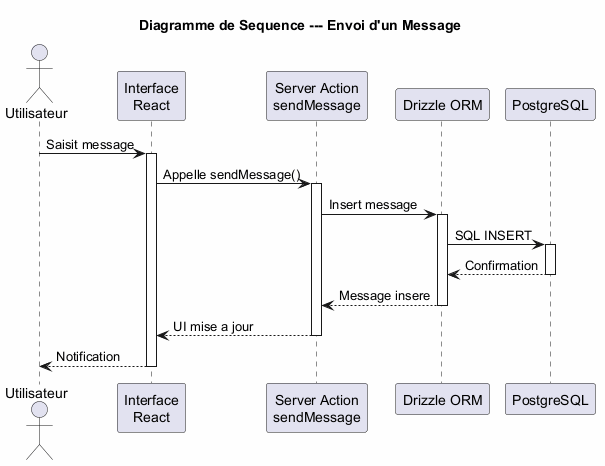
\includegraphics[width=0.95\textwidth,height=0.70\textheight,keepaspectratio]{assets/sequence.png}
\caption{Diagramme de S\'equence --- Envoi d'un Message}
\label{fig:sequence}
\end{figure}

L'utilisateur \'emetteur saisit le message via l'interface React. Le composant client appelle l'action serveur qui ins\`ere le message dans la base de donn\'ees via l'ORM. Cette architecture d\'emontre la s\'eparation des pr\'eoccupations entre pr\'esentation, m\'etier et persistance.

\subsection{M\'ethodes Formelles et Langage Z}

Les m\'ethodes formelles (langage Z, B, VDM) utilisent des notations math\'ematiques pour sp\'ecifier, d\'evelopper et v\'erifier des syst\`emes logiciels. Le langage Z, d\'evelopp\'e par Jean-Raymond Abrial, est bas\'e sur la th\'eorie des ensembles et la logique des pr\'edicats.

Ces m\'ethodes n'ont pas \'et\'e utilis\'ees dans ce projet pour plusieurs raisons pragmatiques : le domaine du marketplace web n'est pas critique au sens des syst\`emes embarqu\'es ; la courbe d'apprentissage est \'elev\'ee ; et TypeScript avec Zod fournissent un niveau de v\'erification suffisant (typage statique, validation de sch\'emas).


% ======================== CHAPITRE 5 ========================
\section{Chapitre 5 : La Normalisation}

Les normes sont des apports document\'es contenant des sp\'ecifications techniques destin\'ees \`a \^etre utilis\'ees syst\'ematiquement comme r\`egles ou lignes directrices.

\subsection{La Norme ISO et la Certification ISO 9000}

L'International Organization for Standardization (ISO), cr\'e\'ee en 1947, est une f\'ed\'eration mondiale d'organismes nationaux de normalisation. La norme ISO 9000 traduit la d\'emarche qualit\'e au niveau de l'entreprise. Dans le contexte de SaaS Directory, la gestion documentaire est assur\'ee par la documentation du projet, et la tra\,cabilit\'e est garantie par l'historique Git et les migrations Drizzle num\'erot\'ees (0000 \`a 0003).

\subsection{Les Normes IEEE}

L'Institute of Electrical and Electronics Engineers (IEEE) a d\'efini un ensemble de normes s'int\'eressant aux processus, produits et techniques de base du g\'enie logiciel.

\begin{definitionbox}[title={IEEE Std 12207.0}]
Fixe la signification des termes et choisit les processus prioritaires du cycle de vie du logiciel. Peut \^etre consid\'er\'ee comme un dictionnaire et une liste de v\'erification pour la gestion des projets.
\end{definitionbox}

\begin{definitionbox}[title={IEEE Std 830}]
Recommand\'ee pour les sp\'ecifications des exigences du logiciel. Pourrait \^etre int\'egr\'ee avec les approches de validation par prototype.
\end{definitionbox}

\begin{definitionbox}[title={IEEE Std 1028}]
Pour appliquer la validation et la v\'erification. Norme facilement adaptable \`a tous les probl\`emes.
\end{definitionbox}

\subsection{Normalisation Appliqu\'ee au Projet}

\subsubsection{Normes de Codage}

Le projet respecte des conventions strictes : PascalCase pour les composants React, camelCase pour les fonctions, et kebab-case pour les routes API. Les imports sont organis\'es par groupe : React/Next.js, biblioth\`eques tierces, composants internes, utilitaires.

\subsubsection{Architecture Normalis\'ee}

L'architecture suit le pattern MVC adapt\'e \`a Next.js 16.2.4. Le \textbf{Mod\`ele} est constitu\'e par le sch\'ema Drizzle ORM. La \textbf{Vue} est impl\'ement\'ee par les composants React. Le \textbf{Contr\^oleur} est assur\'e par les actions serveur du framework.

\subsubsection{Gestion Documentaire et Tra\,cabilit\'e}

La gestion documentaire est assur\'ee par plusieurs artefacts : documentation de pr\'esentation et installation, conventions de d\'eveloppement, gestion des d\'ependances avec versions exactes, et messages de commit suivant une convention descriptive.


% ======================== CHAPITRE 6 ========================
\section{Chapitre 6 : Les Tests}

Les tests logiciels constituent une phase critique du cycle de vie du logiciel, visant \`a d\'etecter les erreurs et \`a garantir que le syst\`eme r\'epond aux exigences sp\'ecifi\'ees.

\subsection{Types de Tests et Strat\'egie}

La strat\'egie de tests de SaaS Directory repose sur une pyramide de tests classique.

\subsubsection{Tests Unitaires}

Les tests unitaires sont impl\'ement\'es avec Vitest 4.1.5. Dix fichiers de test couvrent l'authentification, la souscription, le sch\'ema de base de donn\'ees, les actions serveur, et les composants UI.

\subsubsection{Tests d'Int\'egration et End-to-End}

Les tests end-to-end sont r\'ealis\'es avec Playwright 1.59.1. La configuration d\'efinit un projet Chromium avec tracing activ\'e. Les tests end-to-end de la page d'accueil valident le parcours utilisateur critique.

\subsubsection{Pyramide des Tests}

La figure~\ref{fig:test-pyramid} illustre la strat\'egie de tests de SaaS Directory selon le mod\`ele de la pyramide classique.

\begin{figure}[htbp]
\centering
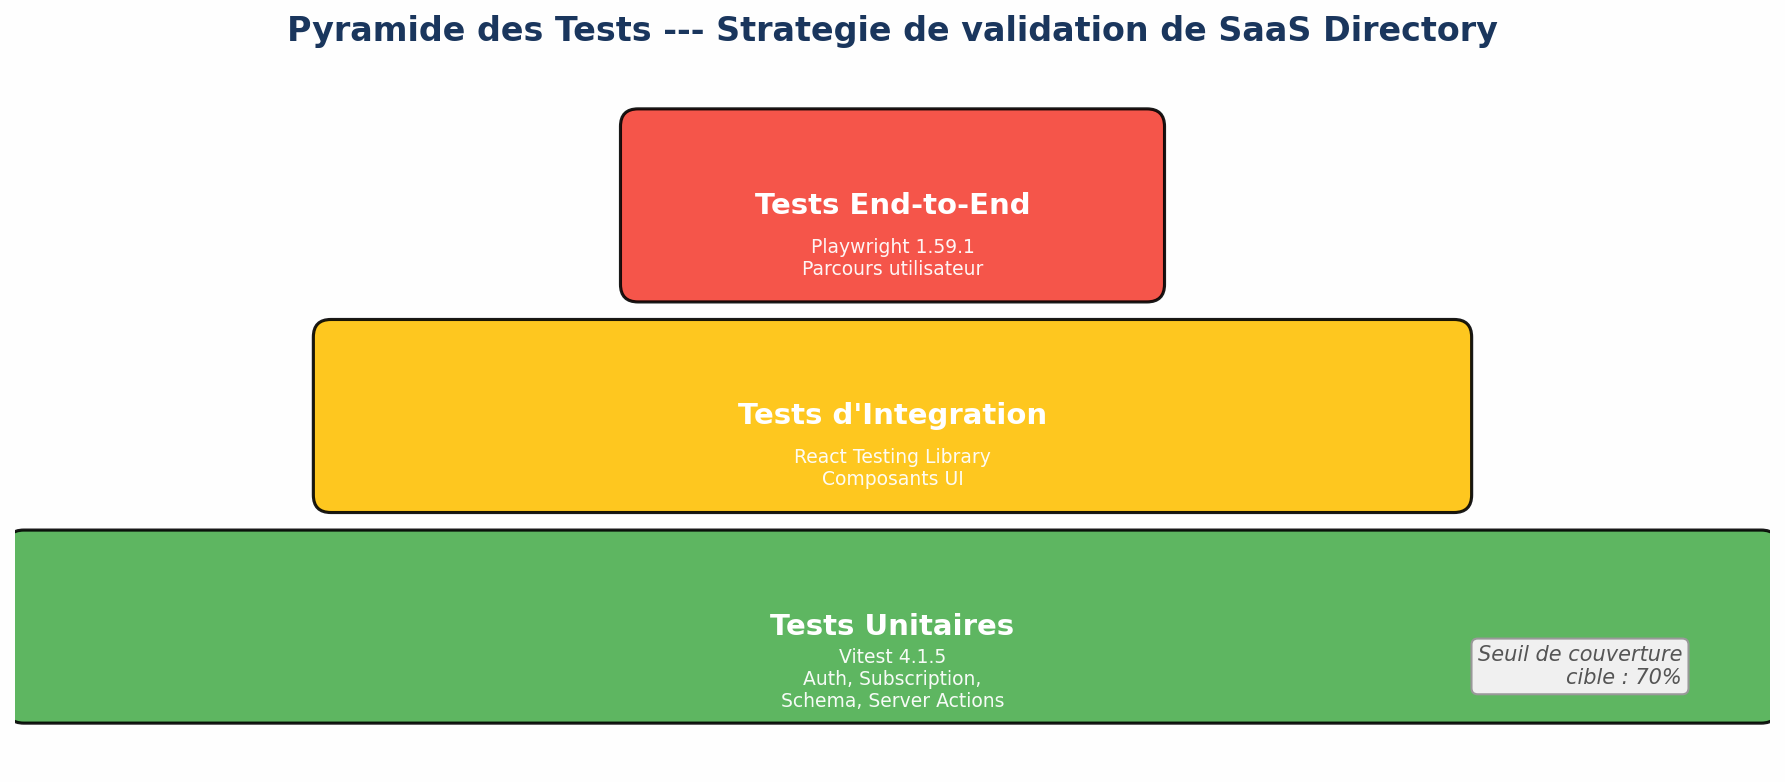
\includegraphics[width=0.85\textwidth,height=0.70\textheight,keepaspectratio]{assets/test_pyramid.png}
\caption{Pyramide des Tests --- Strat\'egie de validation de SaaS Directory}
\label{fig:test-pyramid}
\end{figure}

\subsubsection{Tests de Performance}

La performance est \'evalu\'ee par l'optimisation des requ\^etes Drizzle ORM et la configuration des indexes PostgreSQL. Le projet inclut un script de benchmark pour le cache Redis.

\subsection{Outils et Environnement de Test}

L'environnement de test utilise une base PostgreSQL d\'edi\'ee sur le port 5433. La s\'eparation des environnements (d\'eveloppement, test, production) est assur\'ee par des variables d'environnement d\'edi\'ees.

\subsection{Couverture et R\'esultats}

La couverture de tests cible les fonctions critiques : authentification (cr\'eation de compte, connexion, 2FA), gestion des r\^oles, marketplace (cr\'eation de produit, vote, commentaire), messagerie (envoi, r\'eception), et abonnements (souscription, changement de plan). Les seuils de couverture sont configur\'es avec un minimum de 70\%.


% ======================== CHAPITRE 7 ========================
\section{Chapitre 7 : La Gestion des Projets Logiciels}

La gestion des projets logiciels vise \`a structurer m\'ethodiquement une r\'ealit\'e \`a venir, en appliquant un objectif et des actions \`a entreprendre avec des ressources donn\'ees.

\subsection{Organisation du Projet (WBS, PBS, OBS)}

Trois outils structurants ont guid\'e l'organisation du projet.

Le \textbf{Work Breakdown Structure (WBS)} d\'ecompose le projet en t\^aches hi\'erarchiques : fondations, infrastructure de tests, base de donn\'ees, authentification, fonctionnalit\'es core, et polissage.

Le \textbf{Product Breakdown Structure (PBS)} identifie les livrables : authentification fonctionnelle, profil utilisateur op\'erationnel, marketplace avec votes et commentaires, syst\`eme de messagerie, et abonnements Free/Pro.

Le \textbf{Organizational Breakdown Structure (OBS)} r\'epartit les responsabilit\'es entre les trois d\'eveloppeurs du projet.

\subsection{Planification (GANTT, PERT)}

\begin{figure}[htbp]
\centering
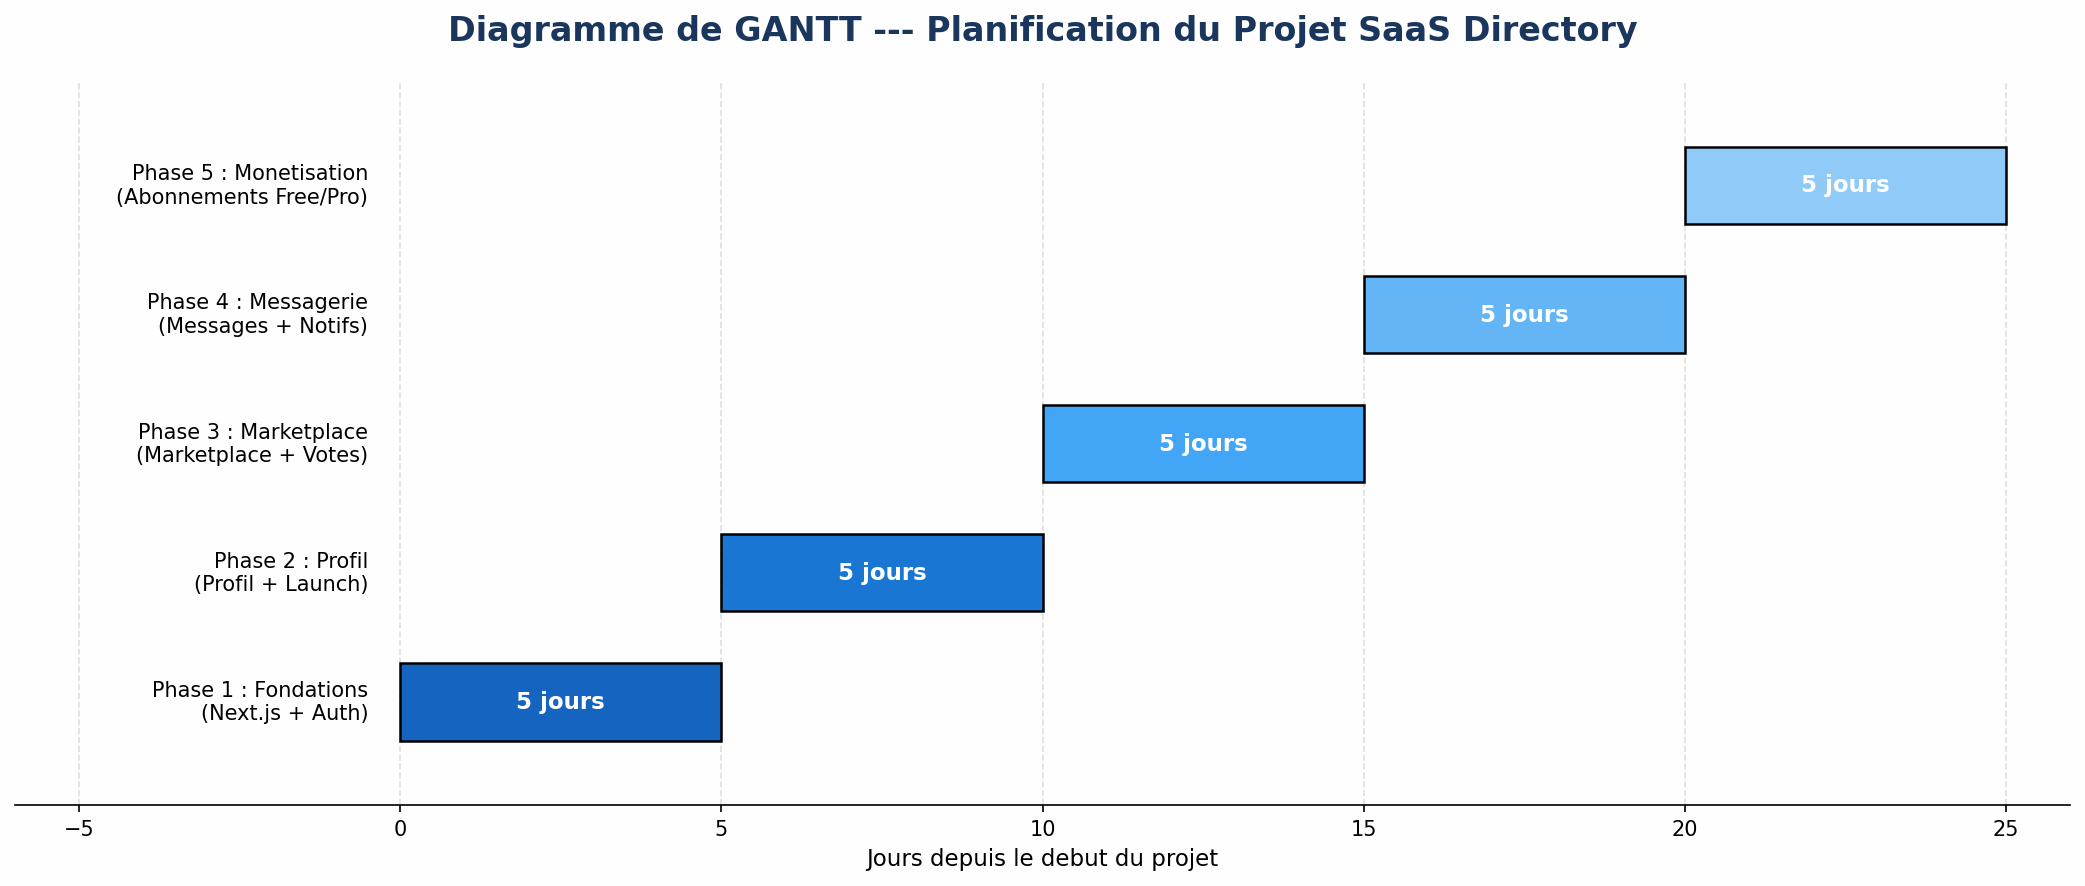
\includegraphics[width=0.95\textwidth,height=0.70\textheight,keepaspectratio]{assets/gantt.png}
\caption{Diagramme de GANTT --- Planification du Projet SaaS Directory}
\label{fig:gantt}
\end{figure}

La figure~\ref{fig:gantt} pr\'esente une planification hypoth\'etique \`a vis\'ee p\'edagogique sur une \'echelle de 130 jours, illustrant le d\'ecoupage type d'un projet web de cette envergure. Le diagramme PERT mod\'elise les d\'ependances entre t\^aches de type ``fin \`a d\'ebut''.

\subsection{Estimation des Co\^uts par COCOMO}

L'estimation des co\^uts d'un projet logiciel est un exercice d\'elicat. Pour contrer les biais classiques (optimisme, n\'eglience technique), nous avons appliqu\'e la m\'ethode COCOMO (COnstructive COst MOdel) de Barry Boehm.

\subsubsection{Taille du Projet}

Le codebase de SaaS Directory compte 12 166 lignes de code r\'eparties sur 108 fichiers TypeScript/TSX, soit approximativement 14 KLOC. R\'epartition principale : application (2 309 LOC), composants (5 234 LOC), utilitaires serveur et librairies (2 957 LOC), tests unitaires et d'int\'egration (1 083 LOC), tests end-to-end (33 LOC).

\subsubsection{Application du COCOMO de Base}

Pour un projet web moderne (Next.js 16.2.4, React 19.2.4, TypeScript 5), nous avons retenu le mode semi-d\'etach\'e. Les coefficients sont $a = 3{,}0$ et $b = 1{,}12$.

\begin{table}[H]
\centering
\caption{Estimation COCOMO de Base --- Mode Semi-D\'etach\'e (14 KLOC)}
\label{tab:cocomo}
\begin{tabular}{@{}lll@{}}
\toprule
\textbf{Param\`etre} & \textbf{Formule / Valeur} & \textbf{R\'esultat} \\
\midrule
Taille du projet & 12 166 LOC $\approx$ 14 KLOC & 14 KLOC \\
Mode de d\'eveloppement & Semi-D\'etach\'e & $a = 3{,}0$ ; $b = 1{,}12$ \\
Effort estim\'e & $E = a \times (\text{KLOC})^b$ & $E \approx 58$ Personnes-Mois \\
Dur\'ee estim\'ee & $D = 2{,}5 \times E^{0{,}35}$ & $D \approx 9{,}5$ mois \\
Taille d'\'equipe th\'eorique & $N = E / D$ & $N \approx 6$ personnes \\
\midrule
\textbf{Taille d'\'equipe r\'eelle} & \textbf{3 d\'eveloppeurs sur 3 semaines} & \textbf{2,3 Personnes-Mois} \\
\bottomrule
\end{tabular}
\end{table}

Ces chiffres constituent une estimation th\'eorique \`a vis\'ee p\'edagogique. En r\'ealit\'e, le projet a \'et\'e r\'ealis\'e par trois d\'eveloppeurs sur environ 2,3 Personnes-Mois (17 jours de d\'eveloppement), illustrant l'\'ecart fr\'equent entre les mod\`eles pr\'edictifs et la r\'ealit\'e des projets acad\'emiques intensifs.


% ======================== CHAPITRE 8 ========================
\section{Chapitre 8 : L'Analyse des Risques}

L'analyse des risques est une composante essentielle de la conduite de projet. Elle vise \`a identifier, \'evaluer et traiter les \'ev\'enements incertains qui pourraient affecter n\'egativement les objectifs.

\subsection{Identification des Risques}

Trois cat\'egories principales de risques ont \'et\'e identifi\'ees.

\subsubsection{Risques Techniques}

Le risque technique majeur r\'eside dans la complexit\'e de Next.js 16.2.4 avec le App Router. Ce framework introduit des breaking changes significatifs par rapport aux versions pr\'ec\'edentes. Un risque secondaire concerne la configuration des relations et indexes Drizzle ORM 0.45.2 + PostgreSQL, qui n\'ecessite une expertise SQL approfondie pour garantir les performances.

\subsubsection{Risques de S\'ecurit\'e}

Les risques de s\'ecurit\'e concernent la protection des donn\'ees utilisateurs et la pr\'evention des attaques. L'injection SQL est mitig\'ee par l'utilisation de Drizzle ORM avec des requ\^etes param\'etr\'ees. Les risques li\'es \`a l'authentification incluent la fuite de tokens JWT et la compromission des sessions. Better Auth 1.6.9 g\`ere nativement plusieurs de ces menaces (expiration des tokens, rotation, rate limiting).

\subsubsection{Risques de Performance}

Le marketplace doit supporter un grand nombre de produits sans d\'egradation du temps de r\'eponse, ce qui n\'ecessite l'optimisation des indexes PostgreSQL et la pagination c\^ot\'e serveur. Le cache Redis est utilis\'e pour r\'eduire la charge sur la base de donn\'ees pour les donn\'ees fr\'equemment acc\'ed\'ees.

\subsection{Analyse et Strat\'egies de Mitigation}

\subsubsection{Mitigation des Risques Techniques}

La mitigation repose sur trois piliers : veille technologique (documentation officielle de Next.js consult\'ee r\'eguli\`erement), tests end-to-end Playwright 1.59.1 pour d\'etecter les r\'egressions, et modularit\'e de l'architecture facilitant le remplacement d'une technologie si elle devient obsol\`ete.

\subsubsection{Mitigation des Risques de S\'ecurit\'e}

La s\'ecurit\'e est assur\'ee par plusieurs m\'ecanismes : Better Auth g\`ere la s\'ecurit\'e des sessions (tokens JWT, expiration, rotation) ; les Server Actions valident les entr\'ees utilisateur via Zod 4.4.3 ; et les indexes PostgreSQL acc\'el\`erent les requ\^etes fr\'equentes tout en limitant l'attaque par injection.

\subsubsection{Mitigation des Risques de Performance}

La performance est optimis\'ee par : les indexes PostgreSQL d\'efinis dans le sch\'ema Drizzle, le cache Redis pour les donn\'ees fr\'equemment acc\'ed\'ees (sessions, profils, listes de cat\'egories), et la pagination c\^ot\'e serveur pour le marketplace et la messagerie.

\subsection{Plan de Continuit\'e}

En cas d'incident majeur, plusieurs mesures sont pr\'e vues : restauration depuis les backups PostgreSQL, reconstruction du sch\'ema via les migrations Drizzle (0000 \`a 0003), retour \`a une version stable via Git (branche principale et tags), et documentation technique facilitant l'onboarding d'un nouveau d\'eveloppeur.


% ======================== CHAPITRE 9 ========================
\section{Chapitre 9 : Conduite du Changement}

La conduite du changement est la discipline qui vise \`a accompagner les transformations au sein d'un projet.

\subsection{Nature des Changements}

Plusieurs types de changements ont affect\'e le projet. Les \textbf{changements technologiques} incluent l'ajout de Framer Motion pour les animations, l'int\'egration de Redis pour le cache c\^ot\'e serveur, et l'\'evolution du sch\'ema Drizzle avec les migrations successives. Les \textbf{changements fonctionnels} concernent l'ajout de fonctionnalit\'es : syst\`eme de notifications, \'edition et suppression des commentaires, pagination infinie pour la messagerie. Les \textbf{changements organisationnels} touchent la r\'epartition des t\^aches entre les deux d\'eveloppeurs.

\subsection{Gestion des Versions}

Le contr\^ole de versions est assur\'e par Git avec une strat\'egie de branches structur\'ee. La branche principale constitue la version de production stable. Les branches de fonctionnalit\'es isolent le d\'eveloppement. Les pull requests avec revue de code assurent la qualit\'e avant fusion.

Les migrations Drizzle constituent un m\'ecanisme de gestion du changement au niveau de la persistance. Chaque migration est un fichier SQL versionn\'e (de 0000 \`a 0003) qui peut \^etre appliqu\'ee et revert\'ee. La figure~\ref{fig:evolution} pr\'esente la chronologie de l'\'evolution du sch\'ema.

\begin{figure}[htbp]
\centering
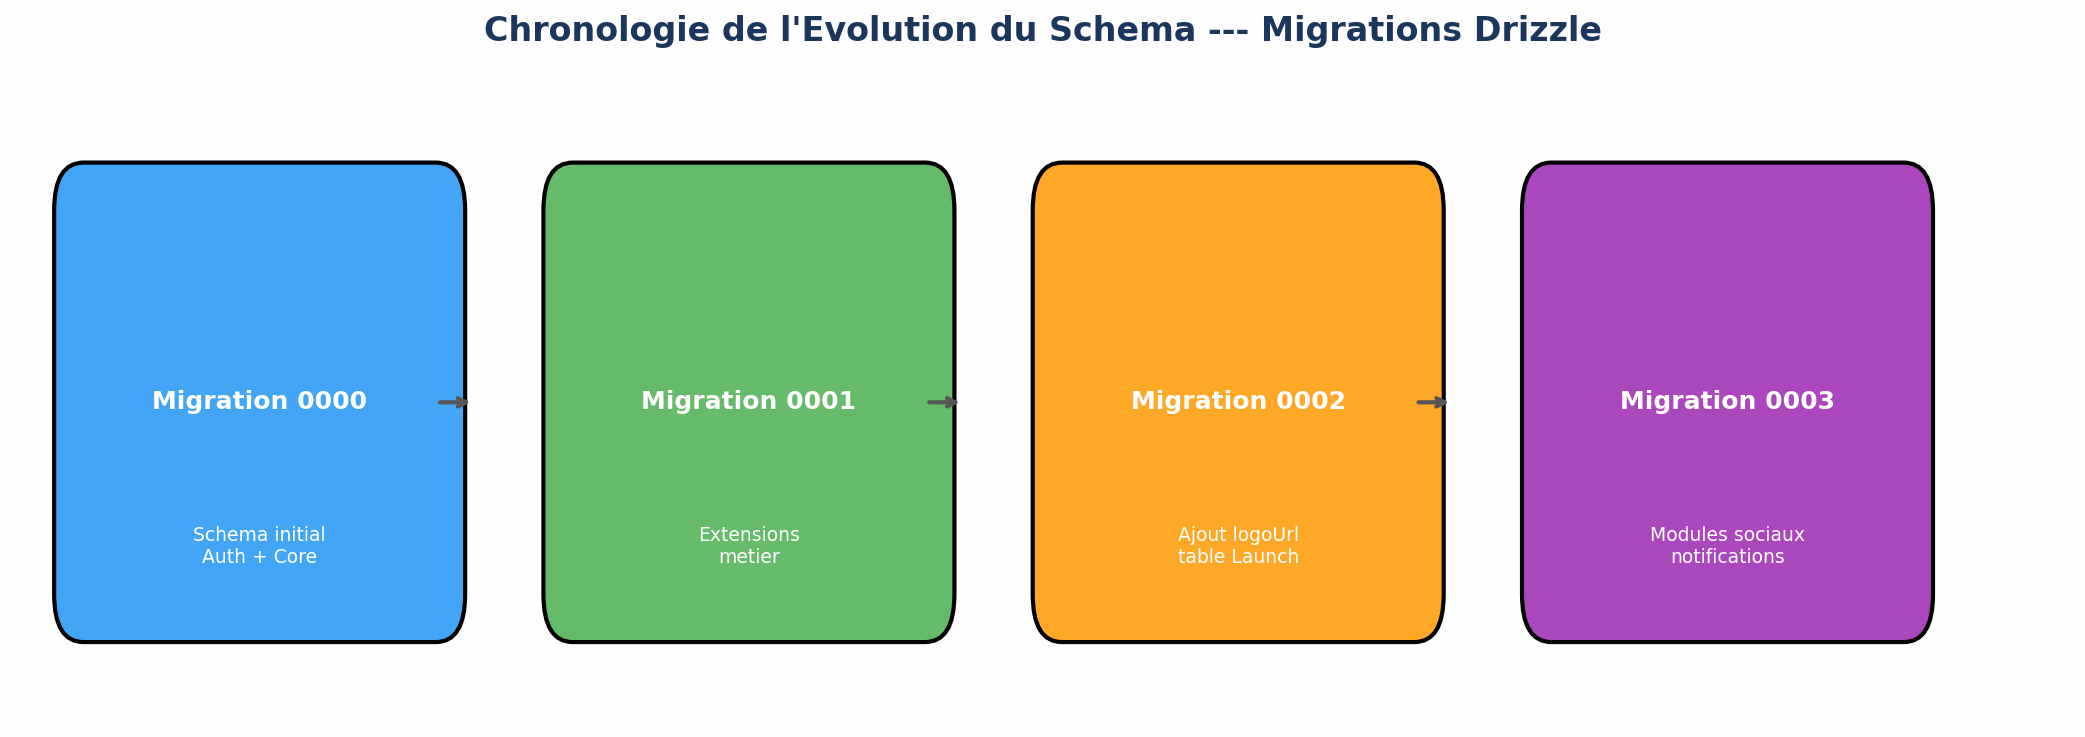
\includegraphics[width=0.95\textwidth,height=0.70\textheight,keepaspectratio]{assets/schema_evolution.png}
\caption{Chronologie de l'\'Evolution du Sch\'ema --- Migrations Drizzle}
\label{fig:evolution}
\end{figure}

Cette approche garantit la coh\'erence du sch\'ema entre les environnements.

\subsection{Adaptation et Communication}

L'architecture modulaire du projet a facilit\'e l'adaptation aux changements. L'ajout du champ logo dans la table des produits (migration 0002) n'a n\'ecessit\'e que la modification du sch\'ema de base de donn\'ees et de l'interface associ\'ee.

La communication autour des changements repose sur plusieurs canaux : la documentation technique maintenue \`a jour, les messages de commit suivant une convention descriptive, et les discussions techniques document\'ees dans les revues de code.
